\section{Teamwork agreement}
The teamwork agreement is an agreement that goes outside the actual project description, and it is defined by the members of the group, based on what each group finds important. Early in the project we therefore wrote down a few key points that were important in terms of teamwork for the group members. The signed teamwork agreement can be seen in \autoref{fig:teamworkagreement}. We broke the agreement into three parts, delivery, wellbeing and learning. The delivery part contains all the points concerning the effort everyone is to put in, and what we're expecting in terms of quality and quantity of work. In the wellbeing section we wrote down what kind of atmosphere and leadership we wanted, as well as any social additions, like eating lunch together each wednesday. In the last section, learning, we wrote down how we wanted to deal with feedback and how to achieve good progress throughout the project, while keeping everyone up to speed.

\begin{figure}
	\begin{center}
		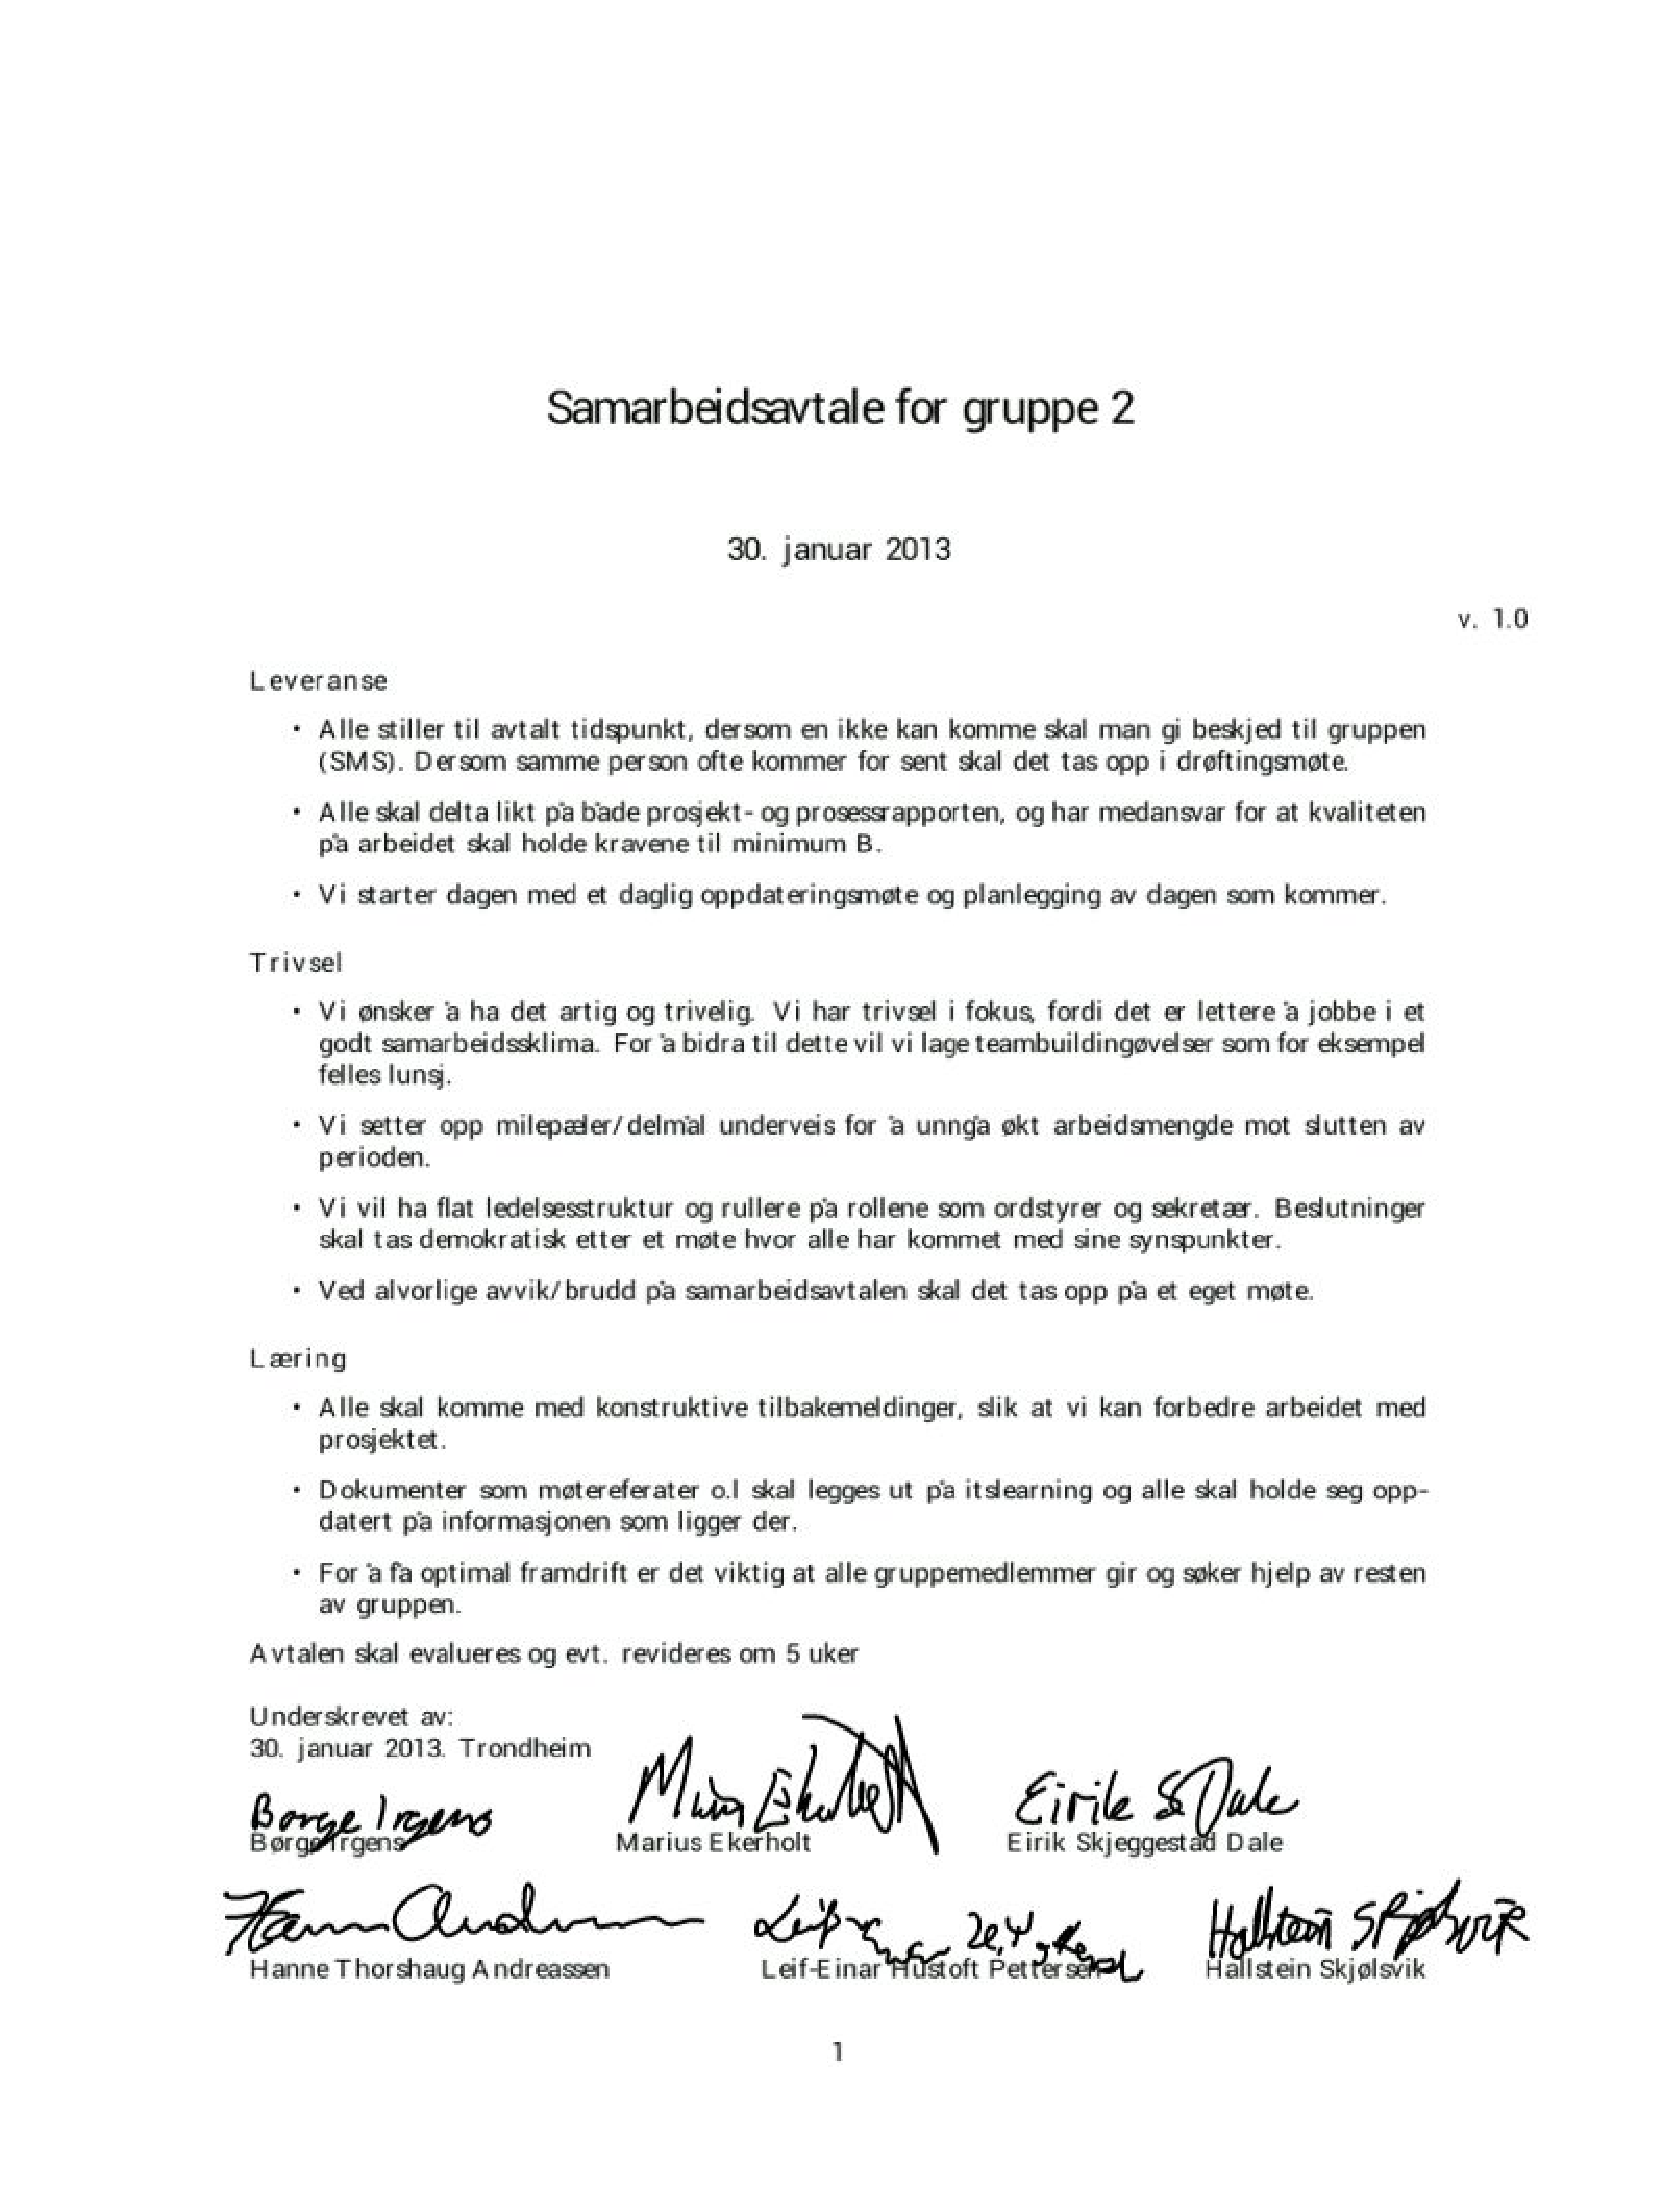
\includegraphics[width=1.0\textwidth]{Figures/teamworkagreement.pdf}
	\end{center}
	\caption[Teamwork agreement]{The signed teamwork agreement}
	\label{fig:teamworkagreement}
\end{figure}